\documentclass[border=4pt]{standalone}
\usepackage{amsmath,amssymb}
\usepackage{tikz}
\begin{document}
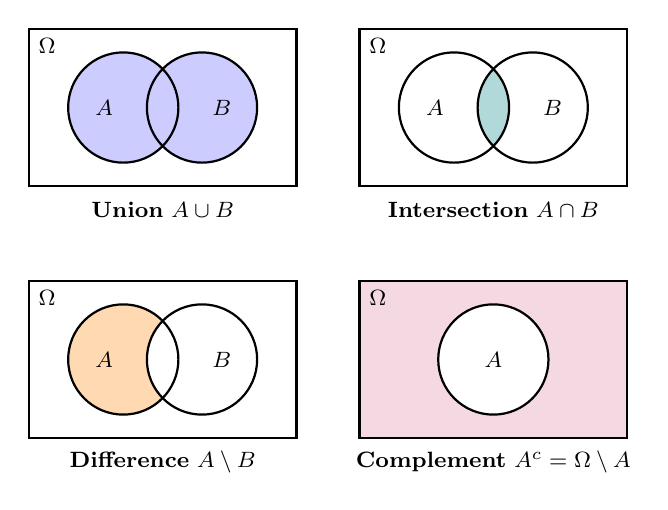
\begin{tikzpicture}[font=\footnotesize]
  % Panel 1: Union
  \begin{scope}[xshift=0cm, yshift=0cm]
    \draw[thick] (-1.2,-1) rectangle (2.2,1);
    \node[anchor=north west] at (-1.2,1) {$\Omega$};
    \fill[blue!20] (0,0) circle (0.7);
    \fill[blue!20] (1,0) circle (0.7);
    \draw[thick] (0,0) circle (0.7) node[left] {$A$};
    \draw[thick] (1,0) circle (0.7) node[right] {$B$};
    \node at (0.5, -1.3) {\textbf{Union} $A \cup B$};
  \end{scope}

  % Panel 2: Intersection
  \begin{scope}[xshift=4.2cm, yshift=0cm]
    \draw[thick] (-1.2,-1) rectangle (2.2,1);
    \node[anchor=north west] at (-1.2,1) {$\Omega$};
    \begin{scope}
      \clip (0,0) circle (0.7);
      \fill[teal!30] (1,0) circle (0.7);
    \end{scope}
    \draw[thick] (0,0) circle (0.7) node[left] {$A$};
    \draw[thick] (1,0) circle (0.7) node[right] {$B$};
    \node at (0.5, -1.3) {\textbf{Intersection} $A \cap B$};
  \end{scope}

  % Panel 3: Difference
  \begin{scope}[xshift=0cm, yshift=-3.2cm]
    \draw[thick] (-1.2,-1) rectangle (2.2,1);
    \node[anchor=north west] at (-1.2,1) {$\Omega$};
    \begin{scope}
      \fill[orange!30] (0,0) circle (0.7);
      \clip (1,0) circle (0.7);
      \fill[white] (0,0) circle (0.7);
    \end{scope}
    \draw[thick] (0,0) circle (0.7) node[left] {$A$};
    \draw[thick] (1,0) circle (0.7) node[right] {$B$};
    \node at (0.5, -1.3) {\textbf{Difference} $A \setminus B$};
  \end{scope}

  % Panel 4: Complement
  \begin{scope}[xshift=4.2cm, yshift=-3.2cm]
    \fill[purple!15] (-1.2,-1) rectangle (2.2,1);
    \fill[white] (0.5,0) circle (0.7);
    \draw[thick] (-1.2,-1) rectangle (2.2,1);
    \node[anchor=north west] at (-1.2,1) {$\Omega$};
    \draw[thick] (0.5,0) circle (0.7) node {$A$};
    \node at (0.5, -1.3) {\textbf{Complement} $A^c = \Omega \setminus A$};
  \end{scope}
\end{tikzpicture}
\end{document}